\documentclass{article}

\usepackage{graphicx}
\usepackage{tikz}
\usepackage{tikzsymbols}
\usetikzlibrary{calc,patterns,shapes.geometric}
\pagestyle{empty}
\usepackage[margin=0pt]{geometry}
\geometry{papersize={14in,12in}}

\def\centerarc[#1](#2)(#3:#4:#5){\draw[#1] ($(#2)+({#5*cos(#3)},{#5*sin(#3)})$) arc (#3:#4:#5);}

\begin{document}
	\begin{figure}
		\centering
		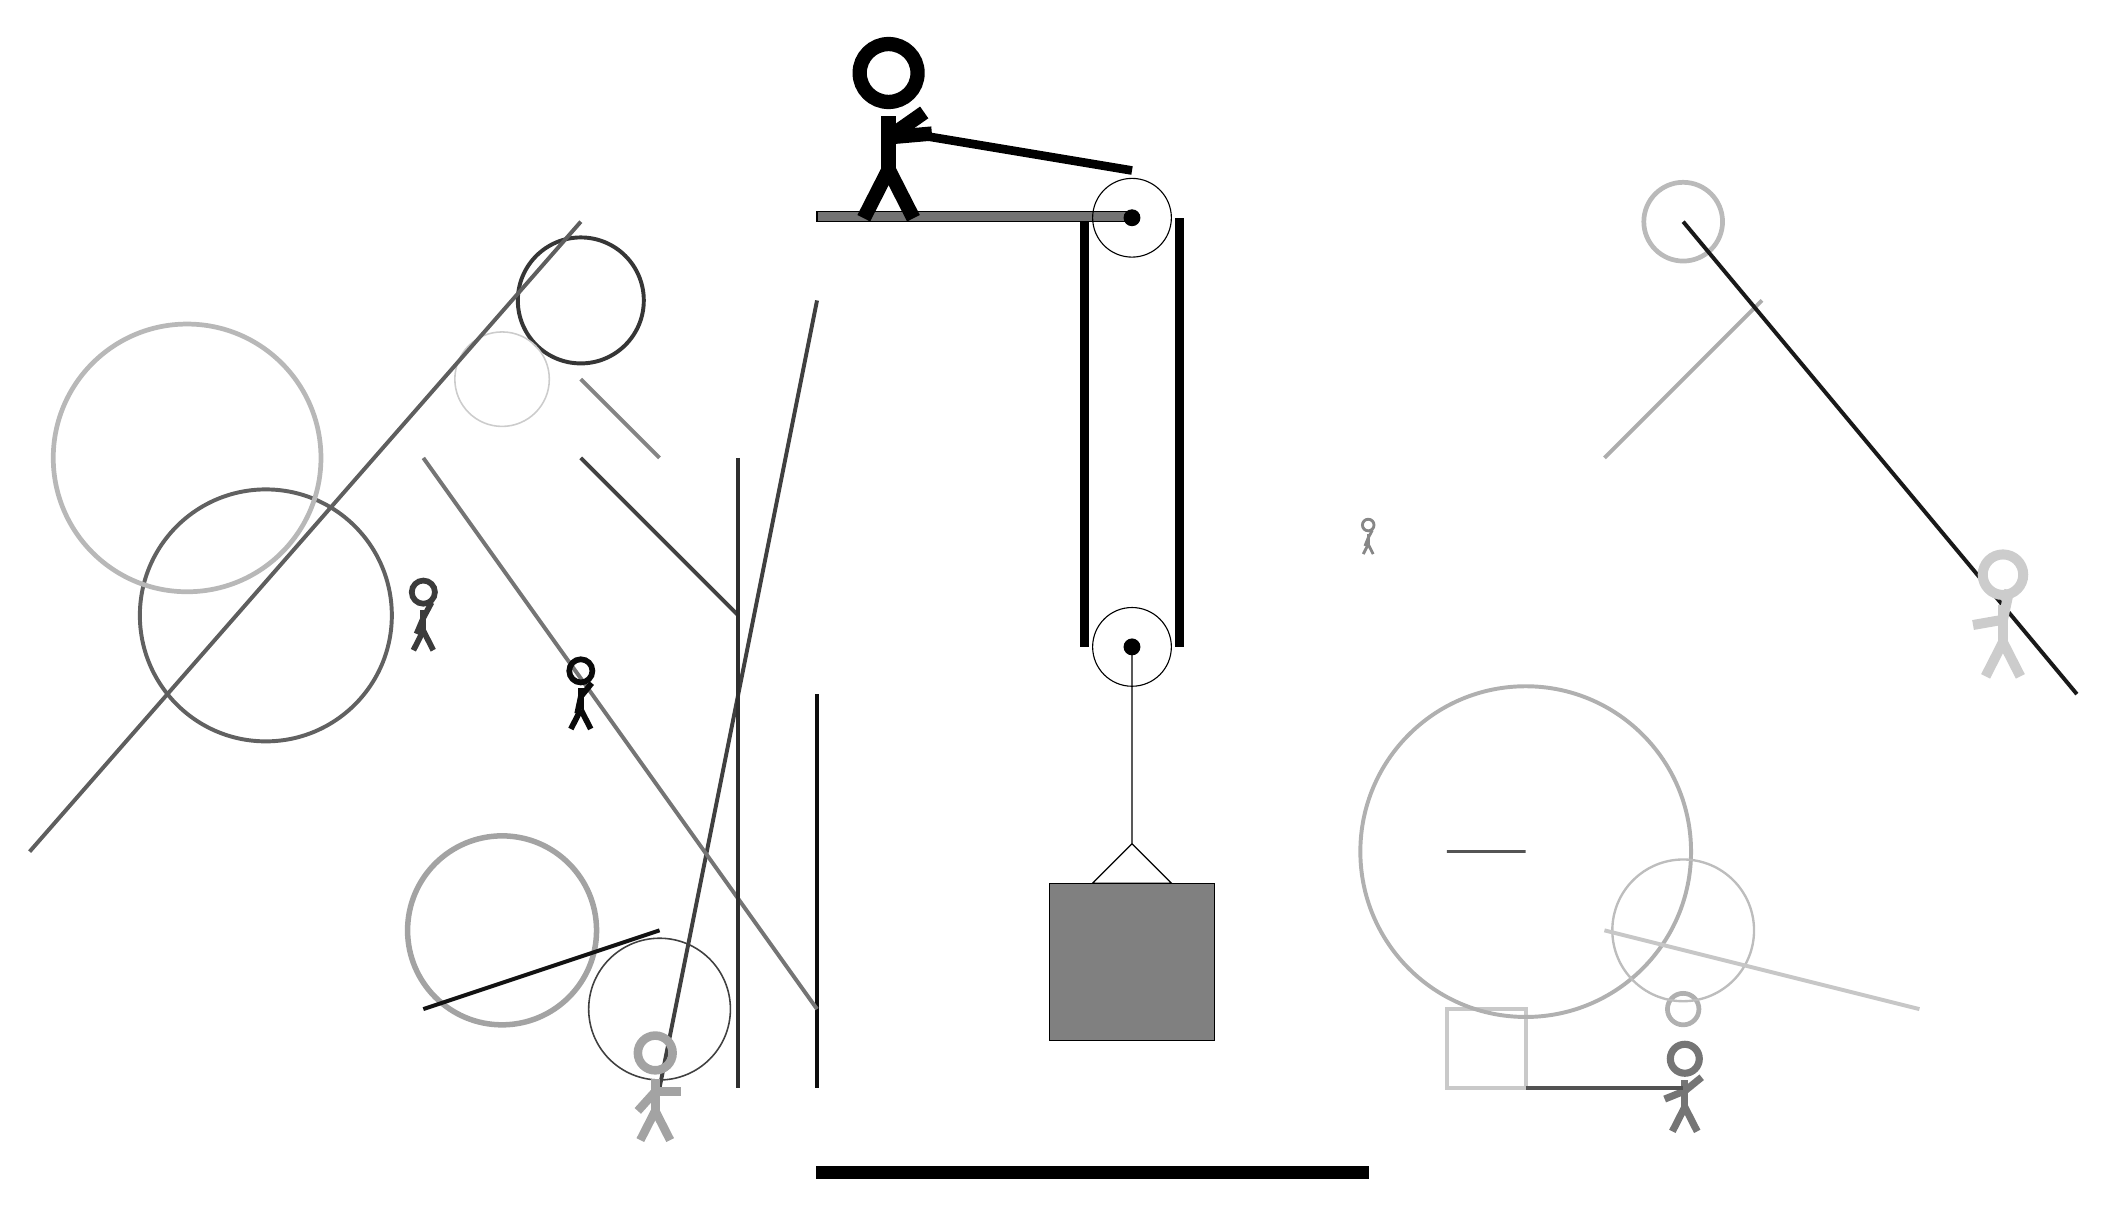
\begin{tikzpicture}
			%%%%% START %%%%%
			
			\draw[fill=black!55] (-2, 9) rectangle (2, 9.125);
			
			\draw (2, 3.6) circle (0.5);
			\draw[fill=black] (2, 3.6) circle (0.1);
			
			\draw (2, 9.05) circle (0.5);
			\draw[fill=black] (2, 9.05) circle (0.1);
			
			\draw (2, 3.6) -- (2, 1.1) -- (1.5, 0.6) -- (2.5, 0.6) -- (2, 1.1);
			\draw[fill=black!50] (0.95, 0.6) rectangle (3.05, -1.4);
			
			\draw[line width=1.1mm] (1.4, 9) -- (1.4, 3.6);
			\centerarc[line width=1.1mm](2, 3.6)(180:360:0.6);
			\draw[line width=1.1mm](2.6, 3.6) -- (2.6, 9.05);
			\centerarc[line width=1.1mm](2, 9.05)(0:90:0.6);
			\draw[line width=1.1mm](2, 9.65) -- (-1, 10.15);
			
			\draw [line width=0.6mm, color=black!27](9, 9) circle (0.5);
			
			\draw[line width=0.3mm, color=black!67] (6, 1) rectangle (7, 1);
			\draw [line width=0.5mm, color=black!62](-9, 4) circle (1.6);
			\draw [line width=0.5mm, color=black!79](-5, 8) circle (0.8);
			\draw[line width=0.5mm, color=black!21] (6, -1) rectangle (7, -2);
			\draw [line width=0.5mm, color=black!31](7, 1) circle (2.1);
			
			\draw[line width=0.5mm, color=black!32](8, 6) -- (10, 8);
			\draw [line width=0.2mm, color=black!20](-6, 7) circle (0.6);
			\draw [line width=0.6mm, color=black!28](-10, 6) circle (1.7);
			\draw [line width=0.2mm, color=black!75](-4, -1) circle (0.9);
			\draw[line width=0.4mm, color=black!95] (-2, 3) rectangle (-2, -2);
			\draw[line width=0.5mm, color=black!63](-5, 9) -- (-12, 1);
			\draw[line width=0.5mm, color=black!48](-4, 6) -- (-5, 7);
			
			\draw[line width=0.5mm, color=black!75](-4, -2) -- (-2, 8);
			\node[line width=0.3mm, color=black!36] at (-4, -2) {\Strichmaxerl[6][48][0]};
			\node[line width=0.5mm, color=black!77] at (-7, 4) {\Strichmaxerl[4][67][62]};
			
			\draw[line width=0.5mm, color=black!54](-2, -1) -- (-7, 6);
			\node[line width=0.5mm, color=black!47] at (5, 5) {\Strichmaxerl[2][68][62]};
			\draw [line width=0.6mm, color=black!31](9, -1) circle (0.2);
			\draw[line width=0.5mm, color=black!74](-3, 4) -- (-5, 6);
			\node[line width=0.7mm, color=black!96] at (-5, 3) {\Strichmaxerl[4][78][51]};
			
			\draw[line width=0.5mm, color=black!82](-3, 6) -- (-3, -2);
			\draw [line width=0.7mm, color=black!36](-6, 0) circle (1.2);
			\draw[line width=0.5mm, color=black!93](-7, -1) -- (-4, 0);
			\node[line width=0.4mm, color=black!54] at (9, -2) {\Strichmaxerl[5][22][39]};
			
			\draw[line width=0.5mm, color=black!68](7, -2) -- (9, -2);
			
			\draw [line width=0.3mm, color=black!26](9, 0) circle (0.9);
			\draw[line width=0.5mm, color=black!90](9, 9) -- (14, 3);
			\node[line width=0.4mm, color=black!20] at (13, 4) {\Strichmaxerl[7][10][78]};
			\draw[line width=0.5mm, color=black!22](8, 0) -- (12, -1);
			
			\node at (-1, 10.15) {\Strichmaxerl[10][-175][35]};
			
			\draw[fill=black] (-2, -3) rectangle (5, -3.15);
			
			%%%%% END %%%%%
		\end{tikzpicture}
	\end{figure}	
\end{document}